\documentclass[11pt,a4paper,titlepage]{report}
\usepackage[utf8]{inputenc}
\usepackage{amsmath}
\usepackage{mathtools}
\usepackage{amsfonts}
\usepackage{amssymb}
\usepackage{graphicx}
\graphicspath{{figures/}}
\usepackage[font=small,labelfont=bf]{caption}
\usepackage{sidecap}
\usepackage{subcaption}
\usepackage[space]{grffile}
\usepackage[left=2cm,right=2cm,top=2cm,bottom=2cm]{geometry}
\usepackage{float}
\usepackage{booktabs}
\usepackage[nottoc]{tocbibind}
\usepackage{wrapfig}
\usepackage[squaren]{SIunits}
\usepackage{units}
\usepackage{array}
\usepackage{xcolor}
\usepackage[export]{adjustbox}
\usepackage{comment}
\usepackage{hyperref}
\usepackage{breakurl}
%\usepackage{url}
%\usepackage[anythingbreaks]{breakurl}
\usepackage[english]{babel}
\usepackage{natbib}
\bibliographystyle{apalike}
\setcitestyle{authoryear,open={(},close={)}}
\usepackage{datetime}
\newdateformat{monthyeardate}{%
  \monthname[\THEMONTH], \THEYEAR}
  %%%%%%%%%%%%%%%%%%%%%%%%%%%%%%%%%%%%%%%%%%%%%%%%%%%%%%% begin the document
\begin{document}
%%%%%%%%%%%%%%%%%%%%%%%%%%%%%%%%%%%%%%%%%%%%%%%%%%%%%%% Title page
\begin{titlepage}
\centering
{\Huge APP MANUAL\par}
\vspace{2cm}

{\Huge Earth Shape Dynamics App (ESD.APP)\par}
\vspace{0.5cm}

{\Large version 07.03.19\par}
\vspace{2cm}
    
{\Large Written and designed by:\\
\huge M.Sc. Mohammad Reza Ershadi\par}
\vspace{2cm}
    
{\LARGE Head of the project:\\
\huge Prof. Dr. Todd Ehlers\par}
\vspace{1cm}

{\LARGE Special thnaks to:\\
\huge Dr. Byron Adams (river erosion part)\\
\huge Dr. Mirjiam Schaller (cosmogenic erosion part)\par}
\vspace{2cm}
        
\centering

\includegraphics[width=0.5\textwidth]{ESD_logo.png}\par
\vspace{1cm}

{\LARGE\monthyeardate\today\par}
\vfill    
    
{\large Department of Geoscience\par}
{\large Eberhard Karls Universität Tübingen\par}  
{\large GERMANY}     
\end{titlepage}
%-------------------------------------------------------------------------------
\tableofcontents
\listoffigures
\listoftables
\newpage
%-------------------------------------------------------------------------------
\chapter{ABOUT THE PROGRAM}
This program is designed to make the plotting procedure of climate and surface processes related map easier and faster. The very raw data used in this program are the mean annual precipitation and temperature from echam5. Some extra modeling and calculation were done to calculate the mean catchment river and cosmogenic erosion rate at each pixel. These are the secondary data which are also stored in the program to make the whole procedure faster. The program is written and designed under "MATLAB App Designer" as a stand-alone app.\\
%-------------------------------------------------------------------------------
\chapter{DATA}
\section{Precipitation and Temperature data}

The program uses mean annual precipitation data as an input of the river erosion rate calculations. Same data along with mean annual temperature data are used to generate precipitation and temperature maps.

The program uses "echam5" mean annual data for different geological time period. The original echam precipitation and temperature files are stored as *.txt files in esd01 server:\\
\url{//134.2.5.43/esd01/share/arc/world/data/Climate/echam}\\

These data were modified as below:\\
1- All the pixels higher than 75\degree N are deleted.
2- All the pixels lower than 60\degree S are deleted. 
3- All the data from oceans and seas are masked.\\

The program only uses the modified version of data files including 26119 pixels. These data are stored in the path below as "PrecipitationData" and "TemperatureData" folders.\\
\url{//134.2.5.43/esd01/data/mershadi/model_runs/Intsall_ESD_app/DataFiles_7.3.2019}\\

We use the following precipitation and temperature data:\\
1- Pliocene (PL)\\
2- Last Glacial Maximum (LGM)\\
3- Mid Holocene (MH)\\
4- Pre-Industry (PI)\\
5- Present Day (PD)\\ 

\section{Erosion data (BriefData)}

The program models river erosion rate and cosmogenic erosion rate by considering several parameters. Depends on the time duration between the initial and final time period, river length, initial rock uplift rate, and bedrock detachment, 360 different conditions and combinations are possible. At the moment 167 different conditions are modeled and available in the program.\\

The outputs of this part for every single condition are three matrices:\\
1- The river erosion rate matrix\\
2- The cosmogenic erosion rate matrix\\
3- The knickpoint shift matrix\\

The river erosion rate and knickpoint shift data have "dx" (distance spacing) of $\frac{length}{1000}$ meters and "dt" (time spacing) of 5 years. This process stops if the river erosion rate reaches a new steady state (less than 1\% of the initial rock uplift rate) or if the model reaches half a million years. This is a very time-consuming process.\\

In order to calculate the cosmogenic erosion rate, the river erosion rate as an input is used. Since the optimized time resolution to calculate cosmogenic erosion rate is 100 years, the time resolution of river erosion rate and knickpoint shift are also considered as 100 years (the river erosion rate and knickpoint shift were calculated every 5 years but only the data at 100 years were extracted). Therefore all the stored data have same time resolution (dt = 100 years).\\

To make the program faster and smaller, the 3 big matrices mentioned above were combined to a small optimized matrix which is the necessary input data for the program. The new matrix only stores the important data from the 3 big matrices (26119 rows which are the number of pixels and only 313 columns). The header of these columns is available in the appendix of this manual (Chapter \ref{sec:apndx}). These new matrices are the second part of the data files of the program. We call them "BriefOutput" or "BriefData". These files are stored in the path below:\\
\url{//134.2.5.43/esd01/data/mershadi/model_runs/Intsall_ESD_app/DataFiles_7.3.2019/BriefData}\\


\section{Extra data}

This folder includes some extra data that program uses to make the things faster and easier.\\
1- Coastlines (*.mat)\\
2- Country borders (*.mat)\\
3- Latitude, longitude and altitude of each pixel (*.mat)\\
4- Cosmogenic sample points and their response time values (*.xlsx)\\
5- Cosmogenic constant factors for each pixel (*.txt)\\
6- LGM ice cover locations (*.nc)\\
7- This manual file (*.pdf)\\

These files are stored in the path below:\\
\url{//134.2.5.43/esd01/data/mershadi/model_runs/Intsall_ESD_app/DataFiles_7.3.2019/ExtraData}\\

\section{Using the data}

Do not forget: after installing the program on your OS, you have to copy all the for mentioned data in the installation path on your computer. They are located in the path below:\\
\url{//134.2.5.43/esd01/data/mershadi/model_runs/Intsall_ESD_app/DataFiles_7.3.2019}\\
%-------------------------------------------------------------------------------
\chapter{The PROGRAM}

\section{Interface}
The program is divided into ten main panels. Some of these panels are divided into some sub-panels. Figure \ref{fig:interface} shows the main interface of the program, all the panels, and sub-panels.

\begin{figure}[H]
    \centering
    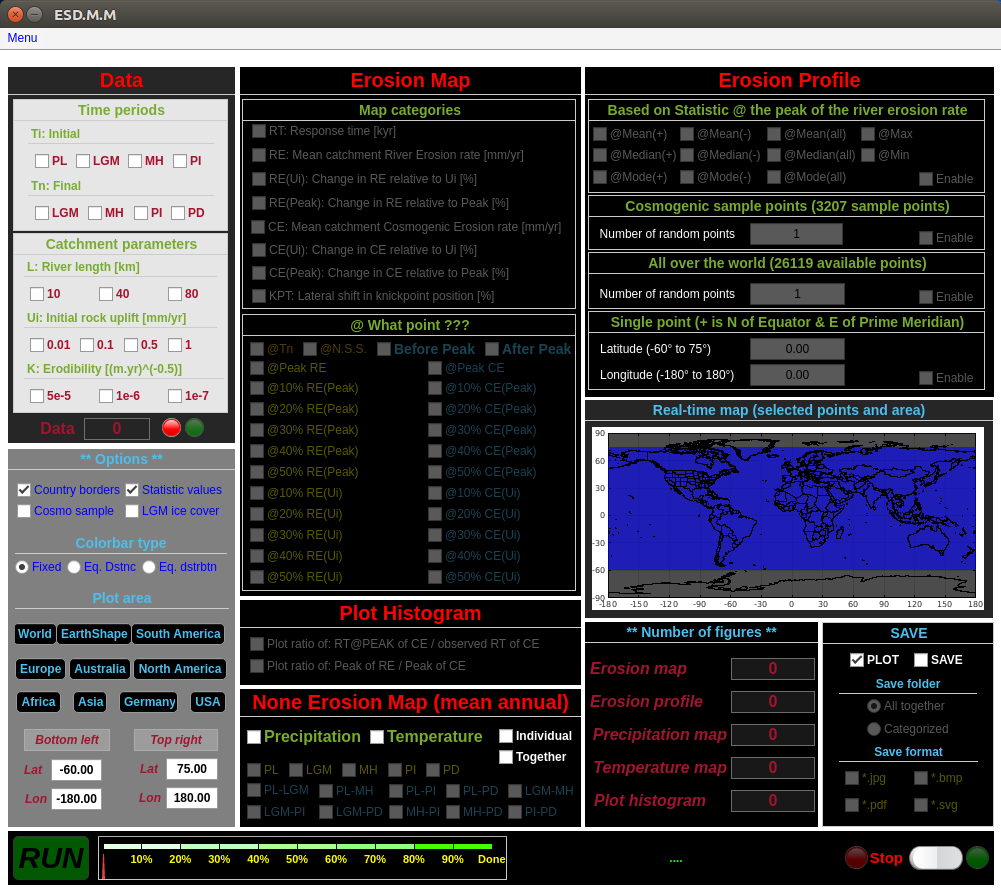
\includegraphics[width=1\textwidth]{mainscreen.png}
    \caption[Interface of the program]{Interface of the program}
    \label{fig:interface}    
\end{figure}

\section{Data panel}
If you want to plot any kind of erosion map or erosion profile, you have to select your data file by choosing the time period and catchment parameters. If the data related to chosen parameters are available, the red light in the data panel turns to green and you see how many data is available based on your choices (figure \ref{fig:datapanel}). As soon as the program find at least one data, the "erosion map" panel, the "histogram" panel and the "enable" checkboxes for "erosion profile" panel will be active.

\begin{figure}[H]
    \centering
    \begin{subfigure}[H]{0.2\textwidth}
        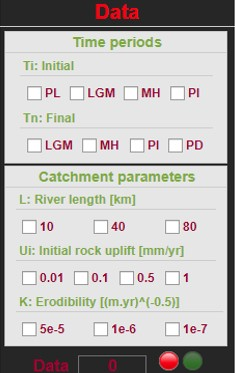
\includegraphics[width=\textwidth]{data1.jpg}
        \caption{No selected data}
    \end{subfigure}
    \quad
    \begin{subfigure}[H]{0.2\textwidth}
        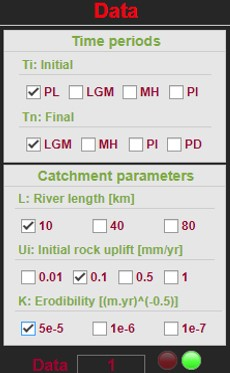
\includegraphics[width=\textwidth]{data2.jpg}
        \caption{One selected data}
    \end{subfigure}
    \quad
    \begin{subfigure}[H]{0.2\textwidth}
        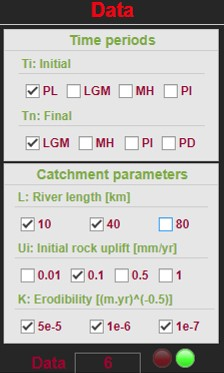
\includegraphics[width=\textwidth]{data3.jpg}
        \caption{Six selected data}
    \end{subfigure}
    \quad
    \begin{subfigure}[H]{0.2\textwidth}
        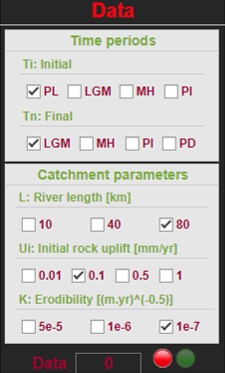
\includegraphics[width=\textwidth]{data4.jpg}
        \caption{Data not available}
    \end{subfigure}\\
    \caption[The data panel]{The data panel}
    \label{fig:datapanel}    
\end{figure}

\section{Options panel}

\begin{wrapfigure}{r}{0.30\textwidth}
    \vspace{-30pt}
  \begin{center}
    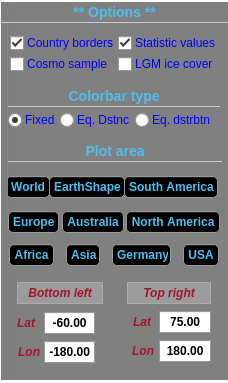
\includegraphics[width=0.30\textwidth]{options1.png}
  \end{center}
  \vspace{-10pt}
  \caption{Options panel}
  \label{fig:options} 
  \vspace{-80pt}
\end{wrapfigure}

In the options panel, you have some choices to apply on your maps (figure \ref{fig:options}). These options are only applicable to erosion and none-erosion map panels (not for profiles or histograms).

\subsection{Country borders}
Add country borders on top of the map.
\subsection{Statistic values}
Only works for erosion maps. Shows some pre-defined statistic parameters for each map. 
\subsection{Cosmo sample}
The location of cosmogenic samples on the maps.
\subsection{LGM ice cover}
Creates a shadow on the location of LGM ice covers on your maps.
\subsection{Color-bar type}
Each map category has a pre-defined color bar and colormap. If you like to limit the color-bar between the min and max values of your map, do not use the "Fixed" option. You have two choices for adaptable color bar. If you want a color bar which is divided into equal distances between min and max, then choose "Eq. Dstnc". In case you like to see your map with equally distributed colors, choose "Eq. dstrbtn". The non-fixed options are very useful when you want to see more details in some specific selected area.
\subsection{Plot area}
You can limit your plotting area by selecting a smaller zone. You can select an area by simply setting the bottom left and top right coordinates of it. You can also use the pre-defined zones to avoid typing coordinates.

\section{Real-time map}
Figure \ref{fig:realmap} shows the real-time map. Any changes you apply, you can see in this map. The blue shadow shows the area you selected to plot your map. By enabling the cosmo sample or LGM ice cover options, you see them as green circles and yellow areas respectively. If you want to plot an erosion profile, the map always shows the location of your selected profile as a red circle.

\begin{figure}[H]
    \centering
    \begin{subfigure}[H]{0.45\textwidth}
        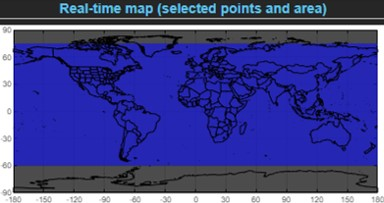
\includegraphics[width=\textwidth]{RM1.jpg}
        \caption{Selected area: world}
    \end{subfigure}
    \quad
    \begin{subfigure}[H]{0.45\textwidth}
        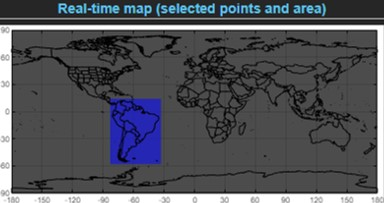
\includegraphics[width=\textwidth]{RM2.jpg}
        \caption{Selected area: South America}
    \end{subfigure}\\
    \begin{subfigure}[H]{0.45\textwidth}
        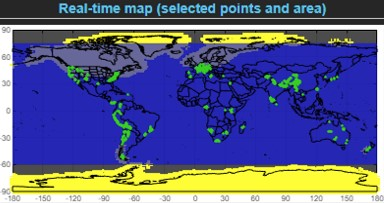
\includegraphics[width=\textwidth]{RM3.jpg}
        \caption{LGM ice cover, Cosmogenic samples}
    \end{subfigure}
    \quad
    \begin{subfigure}[H]{0.45\textwidth}
        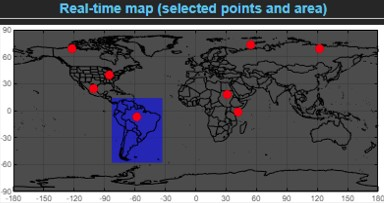
\includegraphics[width=\textwidth]{RM4.jpg}
        \caption{Selected profiles}
    \end{subfigure}\\
    \caption[Real-time map]{Real-time map}
    \label{fig:realmap}    
\end{figure}

\section{Number of figures panel and Run}
Figure \ref{fig:nfigures} shows the "Number of figures" panel. This is an information panel. Here you can see how many separated figures you are about to plot in each category. Figure \ref{fig:runpanel} is the "RUN" panel. If you have nothing to plot (figure \ref{fig:nfigures0}), the RUN button stays off (figure \ref{fig:runpanel0}). As soon as you have at least one map ready to plot (figure \ref{fig:nfigures1}), the RUN button turns on (figure \ref{fig:runpanel1}) and you can plot your selected category. 

\begin{figure}[H]
    \centering
    \begin{subfigure}[H]{0.20\textwidth}
        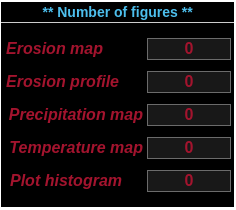
\includegraphics[width=\textwidth]{nfigures1.png}
        \caption{Nothing to plot, RUN off}
        \label{fig:nfigures0}
    \end{subfigure}
    \quad
    \begin{subfigure}[H]{0.20\textwidth}
        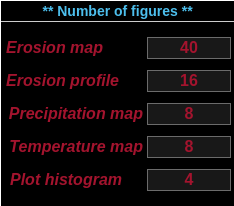
\includegraphics[width=\textwidth]{nfigures2.png}
        \caption{Ready to plot, RUN on}
        \label{fig:nfigures1}
    \end{subfigure}\\
    \caption[Number of figures panel]{Number of figures panel}
    \label{fig:nfigures}    
\end{figure}

\begin{figure}[H]
    \centering
    \begin{subfigure}[H]{0.5\textwidth}
        
\includegraphics[width=\textwidth]{run1.png}
        \caption{RUN button is off}
        \label{fig:runpanel0} 
    \end{subfigure}\\
    \begin{subfigure}[H]{0.5\textwidth}
        
\includegraphics[width=\textwidth]{run2.png}
        \caption{RUN button is on (ready to plot)}
        \label{fig:runpanel1} 
    \end{subfigure}\\
    \caption[RUN panel]{RUN panel}
    \label{fig:runpanel}    
\end{figure}

\section{Save panel}
Figure \ref{fig:savepanel} is the "SAVE" panel. The two checkboxes at top of this panel (plot \& save) tell the program if the user wants to plot the figures, save the figures, or both. You have to select at least one option otherwise, you can not plot (RUN buttons stays off). If you select "PLOT" (figure \ref{fig:savepanel0}), all the chosen figures will pop-up on the screen (but not saved anywhere). As soon as you select the "SAVE" option, the "save folder" sub-panel turns to the active mode (figure \ref{fig:savepanel1}). "All together" option means the user select a folder and the program will save all the figures in that folder. The "categorized" option means the user select a folder but the program will make sub-folders and put each figure in its own sub-folder depending on its type and parameters. Selecting "SAVE" without selecting "PLOT" only saves the figures without showing them on the screen. You can save your plots in four different formats. Please note that saving the figures is very time consuming process.

\begin{figure}[H]
    \centering
    \begin{subfigure}[H]{0.2\textwidth}
        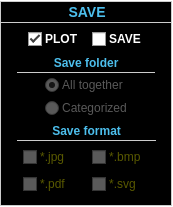
\includegraphics[width=\textwidth]{save1.png}
        \caption{Do not save}
        \label{fig:savepanel0}
    \end{subfigure}
    \quad
    \begin{subfigure}[H]{0.2\textwidth}
        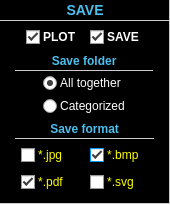
\includegraphics[width=\textwidth]{save2.png}
        \caption{Ready to save}
        \label{fig:savepanel1}
    \end{subfigure}\\
    \caption[Save panel]{Save panel}
    \label{fig:savepanel}    
\end{figure}


\section{None Erosion Map panel}
In this panel, you can plot mean annual precipitation or mean annual temperature maps.
In order to plot non-erosion maps, you do not need to use the data panel. You can directly plot them by selecting the data inside the precipitation panel. Here you have options to plot mean annual maps (yellow checkboxes) or mean annual difference maps (blue checkboxes) which is the difference of mean annual precipitation or temperature between two chosen time periods. You can not select any data (figure \ref{fig:nonerosion0}) unless you choose at least one map category (precipitation or temperature) and at least one plotting type (individual or together) as shown in figure \ref{fig:nonerosion1}.\\

\begin{figure}[H]
    \centering
    \begin{subfigure}[H]{0.45\textwidth}
        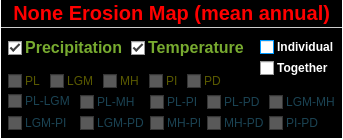
\includegraphics[width=\textwidth]{noneerosion1.png}
        \caption{Time periods are off}
        \label{fig:nonerosion0}
    \end{subfigure}
    \quad
    \begin{subfigure}[H]{0.45\textwidth}
        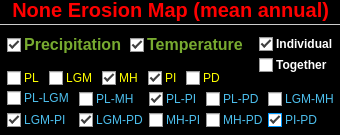
\includegraphics[width=\textwidth]{noneerosion2.png}
        \caption{Time periods are on}
        \label{fig:nonerosion1}
    \end{subfigure}\\
    \caption[None Erosion Map panel\\ ]{None Erosion Map panel\\ }
    \label{fig:nonerosion}    
\end{figure}

\subsection{In one figure / In separated figures}
If you choose two or more than two time-periods from yellow checkboxes, you can put all of them in one page or you can plot each one in a separate page. Also same for the blue checkboxes, but you can not combine blue and yellow options on one page together.

\subsection{Precipitation or Temperature map}
Five yellow check-boxes are designed to plot mean annual precipitation or temperature maps for five time periods. These data are from echam5.

\subsection{Precipitation or Temperature difference map}
The blue checkboxes are designed in order to plot mean annual precipitation or temperature difference between two time periods. These are all the ten possible combinations from the yellow checkboxes.

\section{Erosion profile panel}
This panel is divided into four sub-panels. In order to use the profile panel, you need to select your data from the data panel first. After you select your data, the "Enable" buttons at the right side of each sub-panel turn on and you can choose how you want to select your profile. You are able to select your profiles based on the statistic of the selected data, or pick some random points or give your own coordinate.

\begin{figure}[H]
    \centering
    \begin{subfigure}[H]{0.3\textwidth}
        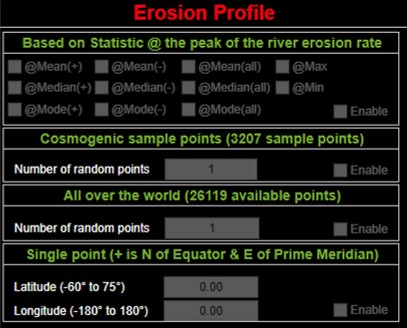
\includegraphics[width=\textwidth]{ep1.jpg}
        \caption{No selected data}
    \end{subfigure}
    \quad
    \begin{subfigure}[H]{0.3\textwidth}
        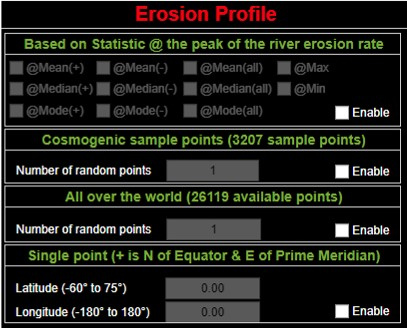
\includegraphics[width=\textwidth]{ep2.jpg}
        \caption{Enable check boxes are active}
    \end{subfigure}
    \quad
    \begin{subfigure}[H]{0.3\textwidth}
        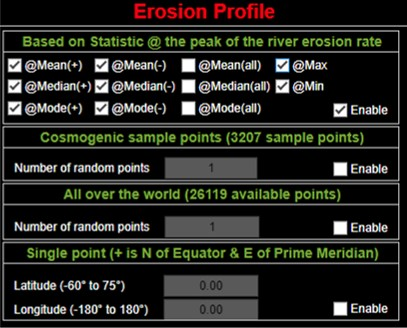
\includegraphics[width=\textwidth]{ep3.jpg}
        \caption{Some profiles are chosen}
    \end{subfigure}\\
    \caption[Erosion profile panel]{Erosion profile panel}
    \label{fig:erosionprofile}    
\end{figure}

\subsection{Select erosion profile based on statistic}
From all the sub-panels for the erosion profiles, the first one (Based on statistic @ the peak of the river erosion rate) might be the most confusing one.\\

\begin{figure}[H]
    \centering
    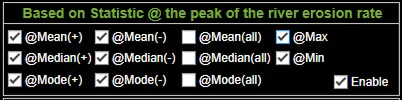
\includegraphics[width=0.4\textwidth]{epstat.jpg}
    \caption[Statistic erosion profile sub-panel]{Statistic erosion profile sub-panel}
    \label{fig:epstat}    
\end{figure}

After you select one data from the data panel, the program finds the associated "BriefData" file. The program looks at a particular column where the river erosion rates at their peak values are stored. All the statistic checkboxes in this sub-panel are calculated from that column (column 42 from BriefData).\\

\begin{figure}[H]
    \centering
    \begin{subfigure}[H]{0.45\textwidth}
        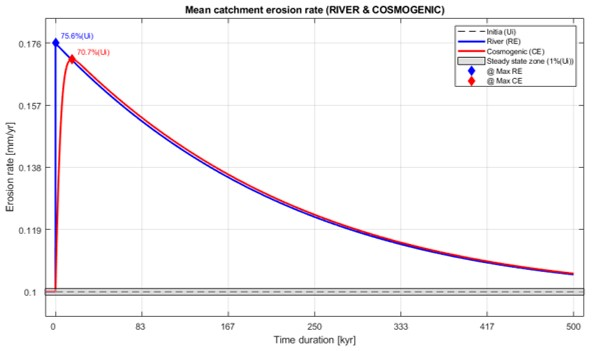
\includegraphics[width=\textwidth]{+profileRC.jpg}
        \caption{A positive (+) profile}
        \label{fig:profiletype_pos}
    \end{subfigure}
    \quad
    \begin{subfigure}[H]{0.45\textwidth}
        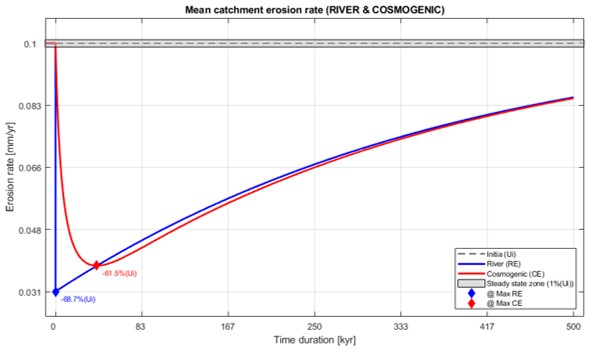
\includegraphics[width=\textwidth]{-profileRC.jpg}
        \caption{A negative (-) profile}
        \label{fig:profiletype_neg}
    \end{subfigure}\\
    \caption[Two possible profile type]{Two possible profile type}
    \label{fig:profiletype}    
\end{figure}

There are only two different types of erosion profile (figure \ref{fig:profiletype}). When the erosion rate jumps and decreases by time to reach to a new steady state (figure \ref{fig:profiletype_pos}). We call these profiles as (+) profiles. The second type is when the erosion rate drops and increases by time to reach to a new steady state (figure \ref{fig:profiletype_neg}). We call these profiles as (-) profiles. Therefore the @Mean(+) check box works like this:\\
The program finds all the pixels which have + profile type. Then it calculates the mean value at the peak of erosion rate. Then the program finds a pixel which has a peak erosion rate value very close to the calculated mean value and plots that. The same procedure is applied for the other checkboxes in this sub-panel.

\subsection{Other erosion profile sub-panels}
You can select as many random points as you want only from the cosmogenic sample points (3207 available sample points). You can also select random points from all the available pixels (26119 pixels). In the last sub-panel, you can give your own coordinate and the program finds the nearest pixel to it.

\begin{figure}[H]
    \centering
    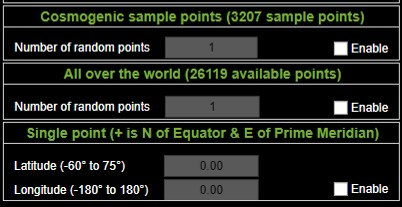
\includegraphics[width=0.4\textwidth]{epothers.jpg}
    \caption[Other erosion profile sub-panels]{Other erosion profile sub-panels}
    \label{fig:epstat}    
\end{figure}

\section{What do you see in an erosion profile}\label{sec:ep}
If you want to use the erosion map panel, it is very important to understand this part. After you plot an erosion profile, you expect to see one of the two types of profiles already explained in the last part (positive (figure \ref{fig:profiletype_pos}) or negative (\ref{fig:profiletype_neg}) profile). Here is an example of what you see in a typical positive and negative erosion profile (figure \ref{fig:ep}).\\

\begin{figure}[H]
    \centering
    \begin{subfigure}[H]{0.8\textwidth}
        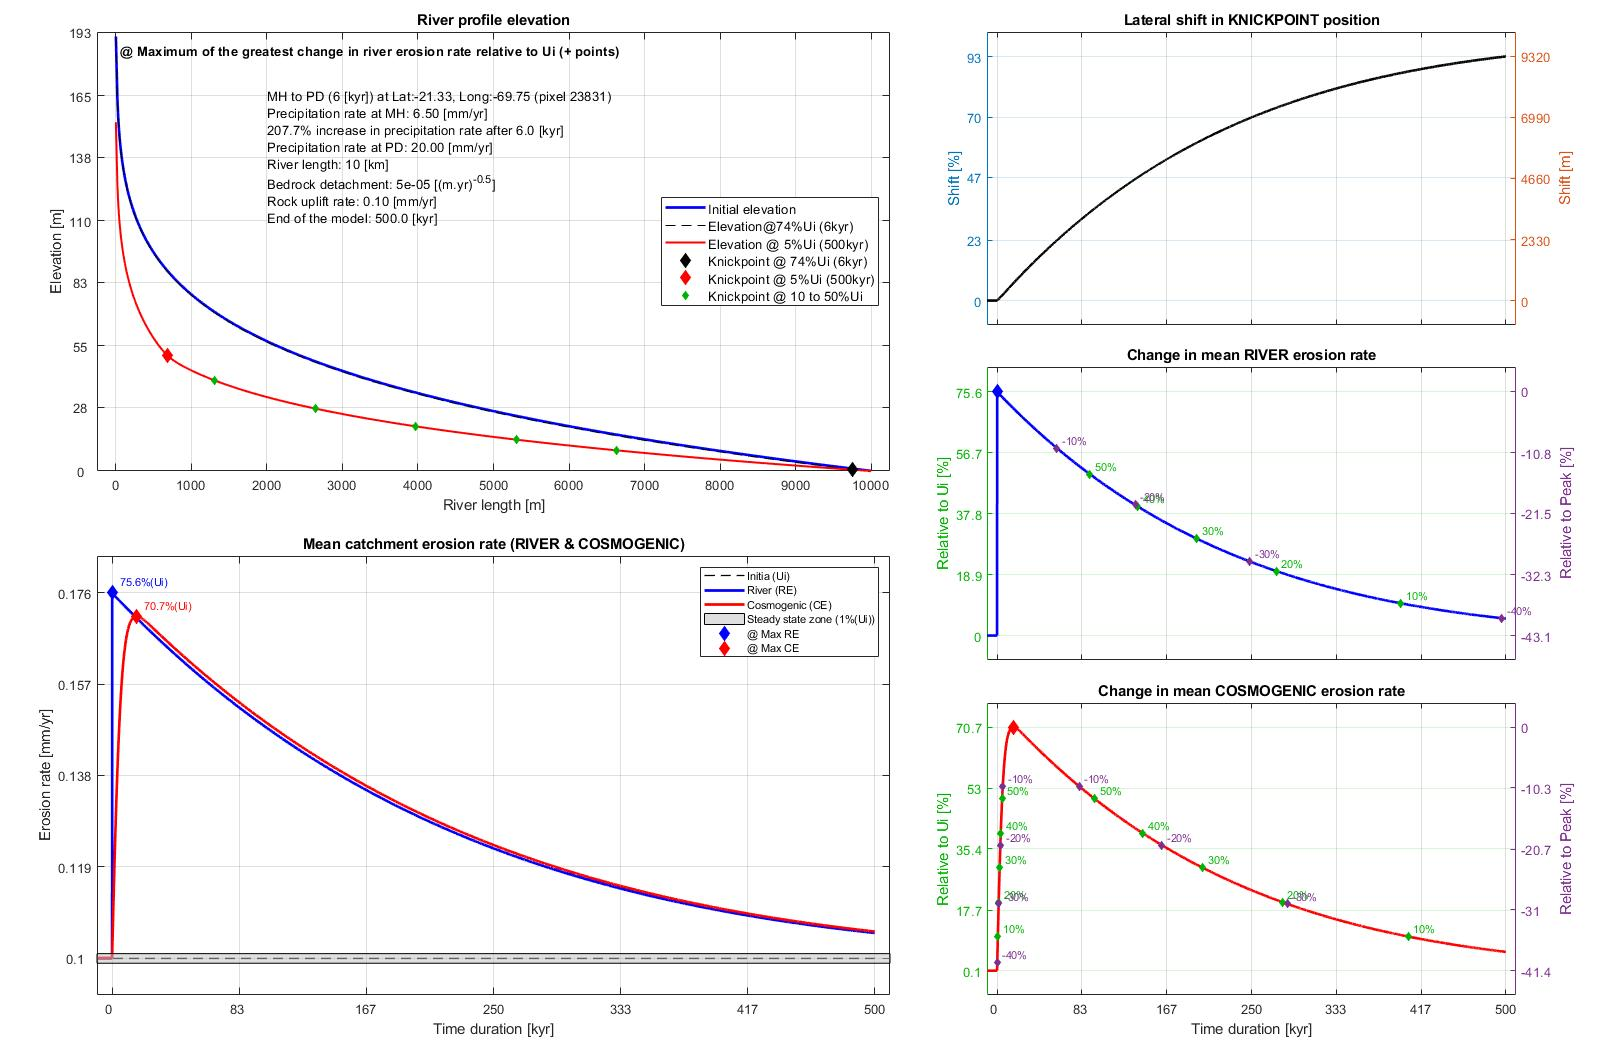
\includegraphics[width=\textwidth]{profile_pmax.jpg}
        \caption{A positive profile}
        \label{fig:ep+}
    \end{subfigure}\\
    \begin{subfigure}[H]{0.8\textwidth}
        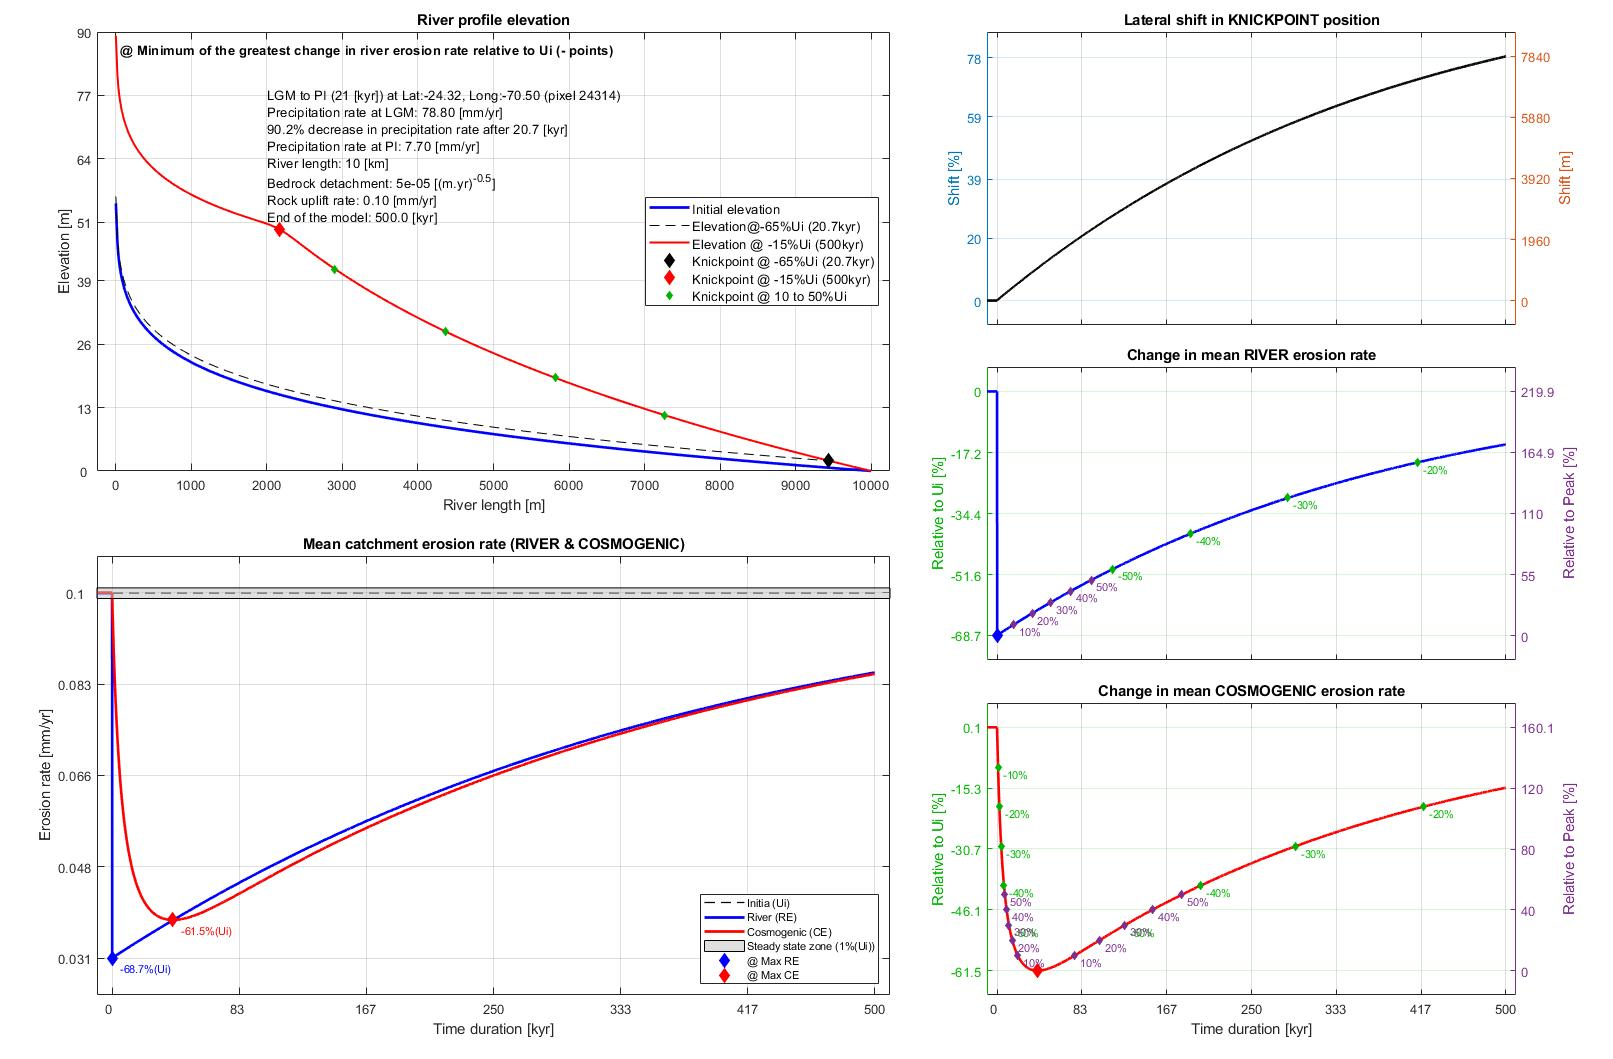
\includegraphics[width=\textwidth]{profile_nmin.jpg}
        \caption{A negative profile}
        \label{fig:ep-}
    \end{subfigure}\\
    \caption[Complete erosion profile]{Complete erosion profile}
    \label{fig:ep}    
\end{figure}

\subsection{River profile elevation (top left subplot)}
The blue line in this figure shows the initial elevation at the beginning of the model and the red line shows the final elevation at the end of the model. The red line can be the elevation line at the new steady state if the model can reach to a new steady state before half a million years. The black dashed line is the elevation at the time duration between the initial and final time period. For example, if the model is between LGM (21000 years) and MH (6000 years), then the black dashed line shows the elevation after 15000 years (we call this time as "tt") but the model will go further if it still not reached to the new steady state. The new steady state defined as if the change between the erosion rate and initial rock uplift rate is less than 1\%.\\

\begin{figure}[H]
    \centering
    \begin{subfigure}[H]{0.45\textwidth}
        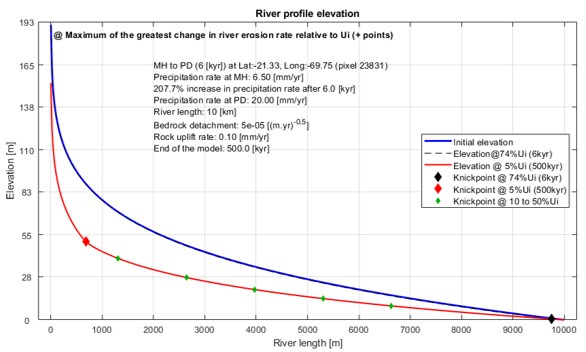
\includegraphics[width=\textwidth]{el_p.jpg}
        \caption{A positive profile}
    \end{subfigure}
    \quad
    \begin{subfigure}[H]{0.45\textwidth}
        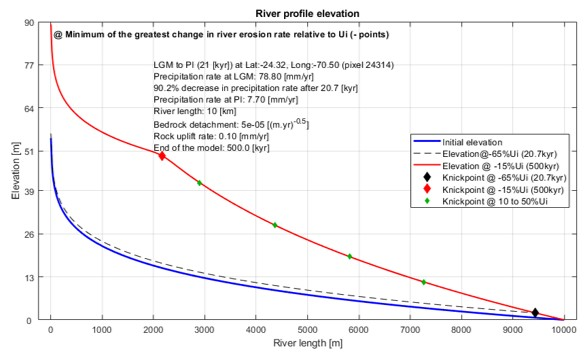
\includegraphics[width=\textwidth]{el_n.jpg}
        \caption{A negative profile}
    \end{subfigure}\\
    \caption[River profile elevation]{River profile elevation}
    \label{fig:elevation}    
\end{figure}

The black diamond and the red diamond show the position of a Nickpoint at "tt" and at the end of the model, respectively. Green diamonds show the Nickpoint positions when the difference between the erosion rate and initial rock uplift rate is at 10\%, 20\%, 30\%, 40\%, and 50\%. You can also find some information about the model and the profile on this figure as text.


\subsection{Lateral shift in knickpoint position (top right subplot)}
The black line in this figure shows how the position of a knickpoint changes by time. The left axis shows the amount of change in percent and the right axis shows the amount of change in meter.\\

\begin{figure}[H]
    \centering
    \begin{subfigure}[H]{0.45\textwidth}
        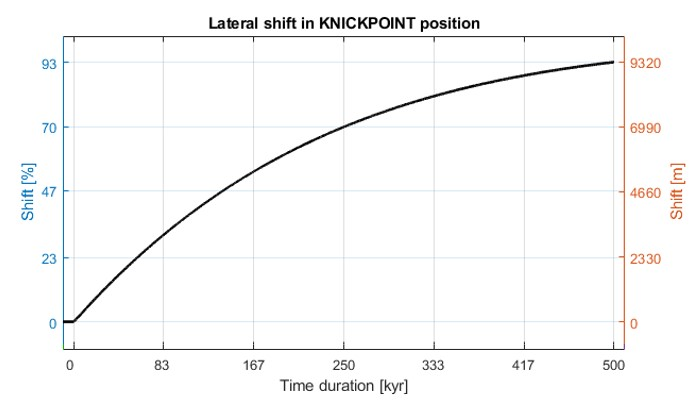
\includegraphics[width=\textwidth]{kp_p.jpg}
        \caption{A positive profile}
    \end{subfigure}
    \quad
    \begin{subfigure}[H]{0.45\textwidth}
        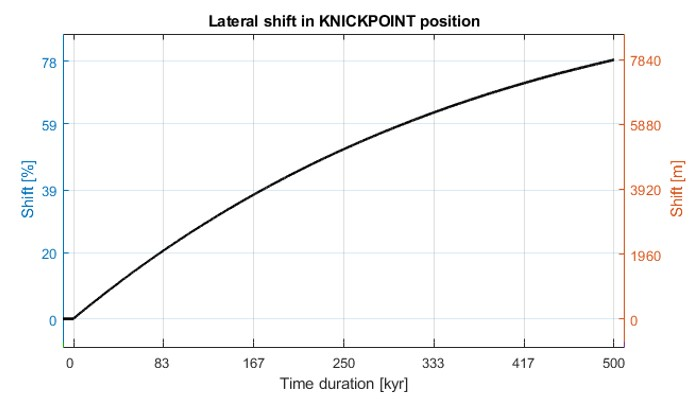
\includegraphics[width=\textwidth]{kp_n.jpg}
        \caption{A negative profile}
    \end{subfigure}\\
    \caption[Lateral shift in knickpoint position]{Lateral shift in knickpoint position}
    \label{fig:knickpoint}    
\end{figure}

\subsection{Mean catchment erosion rate (bottom left subplot)}
This figure shows the mean catchment river erosion rate (blue) and the mean catchment cosmogenic erosion rate (red) in time. The diamonds show the peak values and the percentage next to each diamonds shows the amount of change in erosion rate relative to the initial rock uplift rate.\\

 
\begin{figure}[H]
    \centering
    \begin{subfigure}[H]{0.45\textwidth}
        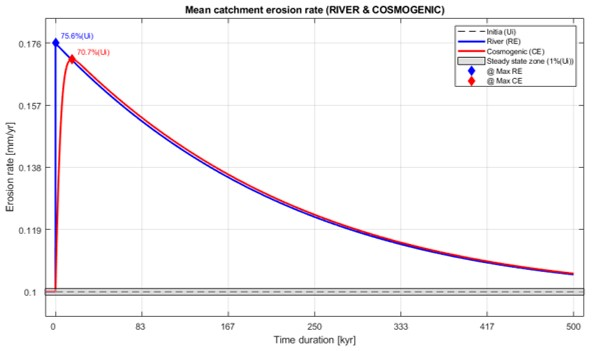
\includegraphics[width=\textwidth]{+profileRC.jpg}
        \caption{A positive profile}
    \end{subfigure}
    \quad
    \begin{subfigure}[H]{0.45\textwidth}
        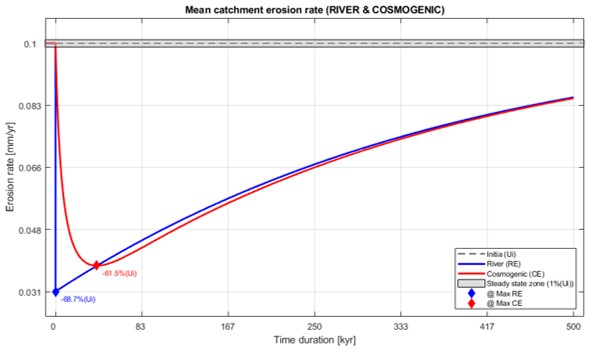
\includegraphics[width=\textwidth]{-profileRC.jpg}
        \caption{A negative profile}
    \end{subfigure}\\
    \caption[Mean catchment erosion rate]{Mean catchment erosion rate}
    \label{fig:erosionrate}    
\end{figure}

The initial rock uplift rate shows as a black dashed line and the gray rectangle around it shows the steady state area which is 1\% difference from the initial rock uplift rate. The model stops before half a million years if the river erosion rate hit the gray rectangle.

\subsection{Change in mean river erosion rate (middle right subplot)}
This figure shows the amount of change in mean catchment river erosion rate relative to the initial rock uplift rate (left axis) and relative to its own peak (right axis). In between, there are some important points which are shown by small green and purple diamonds.

\begin{figure}[H]
    \centering
    \begin{subfigure}[H]{0.45\textwidth}
        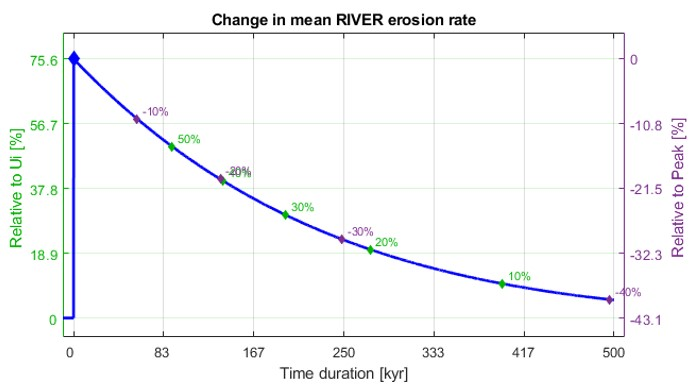
\includegraphics[width=\textwidth]{RE_p.jpg}
        \caption{A positive profile}
    \end{subfigure}
    \quad
    \begin{subfigure}[H]{0.45\textwidth}
        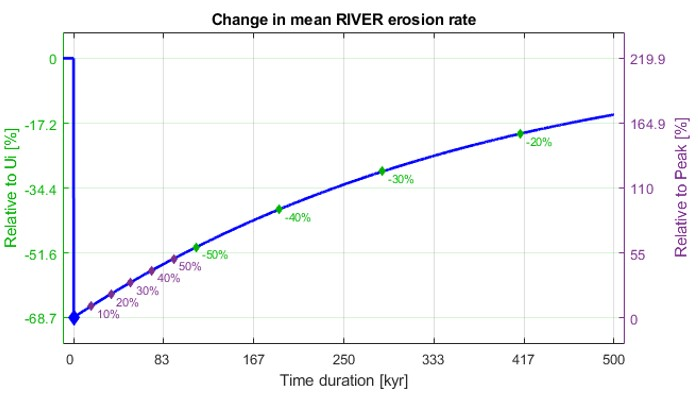
\includegraphics[width=\textwidth]{RE_n.jpg}
        \caption{A negative profile}
    \end{subfigure}\\
    \caption[Change in mean river erosion rate]{Change in mean river erosion rate}
    \label{fig:erosionrate}    
\end{figure}

The green axis in the left side of the figure shows the amount of change in the mean catchment river erosion rate relative to the initial rock uplift rate. The green diamonds are the points when this change reaches to 10\%, 20\%, 30\%, 40\%, and 50\%.\\

The purple axis in the right side of the figure shows the amount of change in the mean catchment river erosion rate relative to its own peak. The purple diamonds are the points when this change reaches to 10\%, 20\%, 30\%, 40\%, and 50\%.\\

\subsection{Change in mean cosmogenic erosion rate (bottom right subplot)}
This figure shows the amount of change in mean catchment cosmogenic erosion rate relative to the initial rock uplift rate (left axis) and relative to its own peak (right axis). In between, there are some important points which are shown by small green and purple diamonds. Since there is usually no vertical jump, these values can be calculated before and after the peak.

\begin{figure}[H]
    \centering
    \begin{subfigure}[H]{0.45\textwidth}
        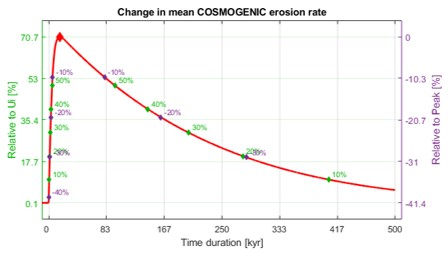
\includegraphics[width=\textwidth]{CE_p.jpg}
        \caption{A positive profile}
    \end{subfigure}
    \quad
    \begin{subfigure}[H]{0.45\textwidth}
        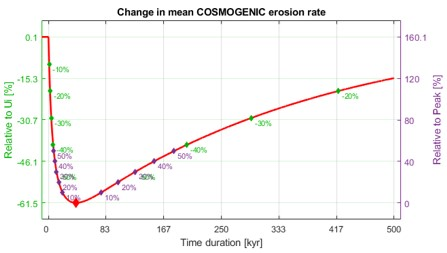
\includegraphics[width=\textwidth]{CE_n.jpg}
        \caption{A negative profile}
    \end{subfigure}\\
    \caption[Change in mean cosmogenic erosion rate]{Change in mean cosmogenic erosion rate}
    \label{fig:erosionrate}    
\end{figure}

The green axis in the left side of the figure shows the amount of change in the mean catchment cosmogenic erosion rate relative to the initial rock uplift rate. The green diamonds are the points when this change reaches to 10\%, 20\%, 30\%, 40\% and 50\% before and after the peak.\\

The purple axis in the right side of the figure shows the amount of change in the mean catchment cosmogenic erosion rate relative to its own peak. The purple diamonds are the points when this change reaches to 10\%, 20\%, 30\%, 40\% and 50\% before and after the peak.\\

\section{Erosion map panel}
It is highly recommended to read the section \ref{sec:ep} before you start using this panel. To use this panel, you need to have at least one selected data from the data panel. As soon as you select at least one data, the map category sub-panel gets active. In order to activate the second sub-panel (@ what point) you need to select at least one map category.\\

\begin{figure}[H]
    \centering
    \begin{subfigure}[H]{0.4\textwidth}
        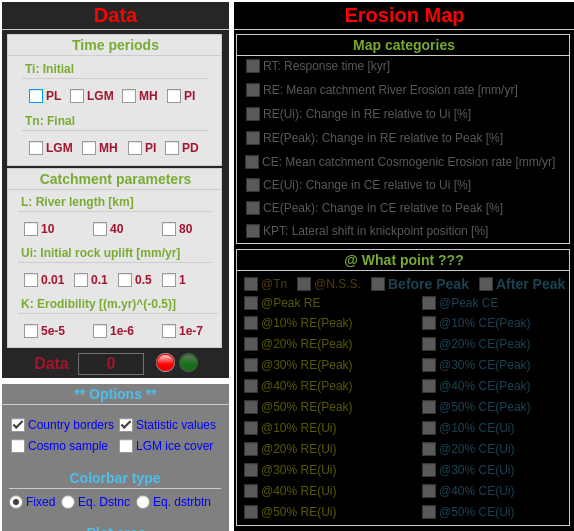
\includegraphics[width=\textwidth]{em1.png}
        \caption{No data selected}
    \end{subfigure}
    \quad
    \begin{subfigure}[H]{0.4\textwidth}
        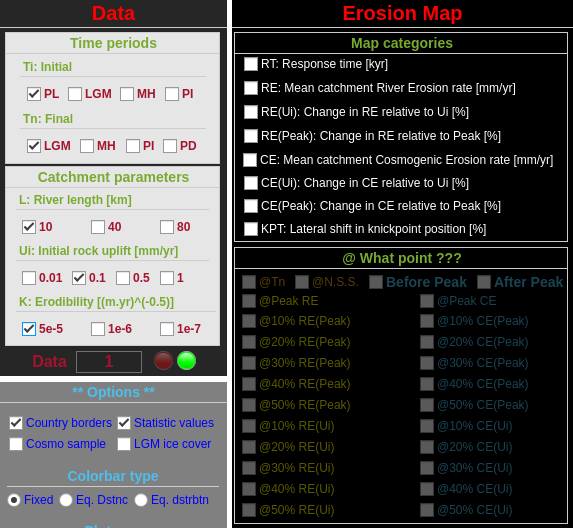
\includegraphics[width=\textwidth]{em2.png}
        \caption{The map category sub-panel is active}
    \end{subfigure}\\
    \caption[Map category activation]{Map category activation}
    \label{fig:mc_active}    
\end{figure}

\subsection{Map category / @ what point}
In "map category" you can select what kind of map or maps you want to generate. This sub-panel is useless without the sub-panel below it (@ what point). These two are working together. As soon as you select at least one map category, then you can choose at what point you want to generate that map.

\begin{figure}[H]
    \centering
    \begin{subfigure}[H]{0.3\textwidth}
        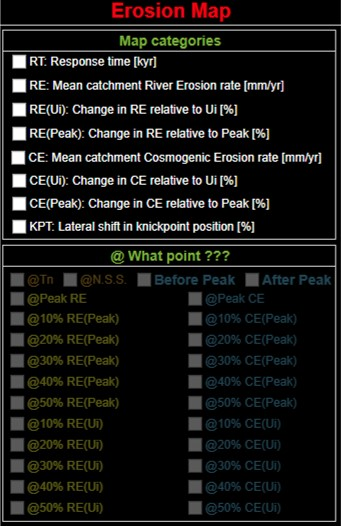
\includegraphics[width=\textwidth]{mcwp1.jpg}
        \caption{No map category selected}
    \end{subfigure}
    \quad
    \begin{subfigure}[H]{0.3\textwidth}
        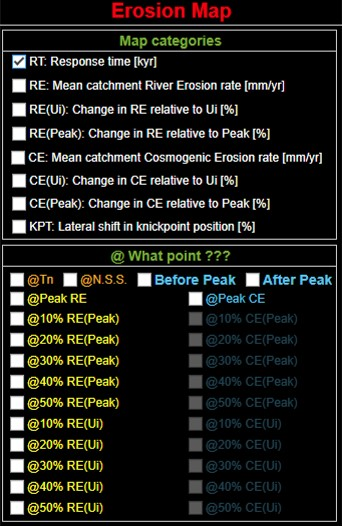
\includegraphics[width=\textwidth]{mcwp2.jpg}
        \caption{Half active}
    \end{subfigure}
    \quad
    \begin{subfigure}[H]{0.3\textwidth}
        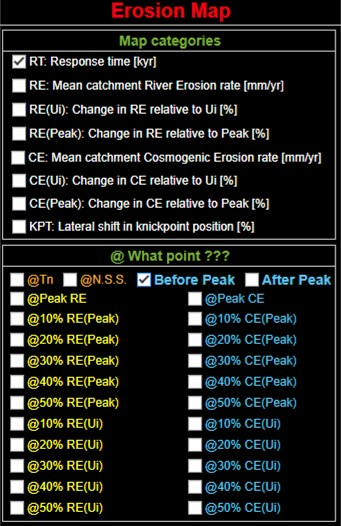
\includegraphics[width=\textwidth]{mcwp3.jpg}
        \caption{All active}
    \end{subfigure}\\    
    \caption["@ what point" sub-panel activation]{@ what point sub-panel activation}
    \label{fig:mc_active}    
\end{figure}

%The following abbreviations are used in the "map category" and the following table:\\
%RT [kyr]: response time.\\
%RE [$\frac{mm}{yr}$]: mean catchment river erosion rate.\\
%RE(UI) [\%]: change in mean catchment river erosion rate relative to UI.\\
%RE(Peak) [\%]: change in mean catchment river erosion rate relative to its own peak.\\
%CE [$\frac{mm}{yr}$]: mean catchment cosmogenic erosion rate.\\
%CE(UI) [\%]: change in mean catchment cosmogenic erosion rate relative to UI.\\
%CE(Peak) [\%]: change in mean catchment cosmogenic erosion rate relative to its own peak.\\
%KPT [\%]: Lateral shift in kickpoint positions.\\
%bp: Before the peak of CE.\\
%ap: After the peak of CE.\\
%UI: Initial rock uplift rate.\\

\begin{table}[H]
\centering
\caption{Some abbreviations and definitions}
\begin{tabular}{l|c|l}
Abbreviation & unit & definition\\
\hline
Ui & [$\frac{mm}{yr}$] & initial rock uplift rate\\
bp & [-] & before peaks\\
ap & [-] & after peak\\
tt & [kyr] & time duration between two geological period\\
RT & [kyr] & response time\\
RE & [$\frac{mm}{yr}$] & mean catchment river erosion rate\\
RE(Ui) & [\%] & change in mean catchment river erosion rate relative to initial rock uplift rate\\
RE(Peak) & [\%] & change in mean catchment river erosion rate relative to its own peak\\
CE & [$\frac{mm}{yr}$] & mean catchment cosmogenic erosion rate\\
CE(Ui) & [\%] & change in mean catchment cosmogenic erosion rate relative to initial rock uplift rate\\
CE(Peak) & [\%] & change in mean catchment cosmogenic erosion rate relative to its own peak\\
KPT & [\%] & lateral shift in kickpoint positions\\
IND & [-] & index\\

\end{tabular}\\
\label{tab:abbr} 
\end{table}

\begin{table}[H]
\centering
\caption{"@ what point" definitions}
\begin{tabular}{l|l|l}
Check box name&definition&label(fig:\ref{fig:RECEhelp2})\\
\hline
\textcolor{orange}{@Tn}&at the end of the model&I\\
\textcolor{orange}{@N.S.S.}&at a new steady state&I\\
\textcolor{yellow}{@Peak RE}&at the peak of RE&A\\
\textcolor{yellow}{@10\% RE(Peak)}&when RE is at 10\% of its peak&D\\
\textcolor{yellow}{@10\% RE(UI)}&when RE is at 10\% of UI&F\\
\textcolor{blue}{@Peak CE}&at the peak of CE&E\\
\textcolor{blue}{@10\% CE(Peak) bp}&when CE is at 10\% and left side of its peak&B\\
\textcolor{blue}{@10\% CE(Peak) ap}&when CE is at 10\% and right side of its peak&H\\
\textcolor{blue}{@10\% CE(UI) bp}&when CE is at 10\% of UI and left side of its peak&C\\
\textcolor{blue}{@10\% CE(UI) ap}&when CE is at 10\% of UI and right side of its peak&G\\
\end{tabular}\\
\label{tab:@RT} 
\end{table}

\begin{figure}[H]
    \centering
    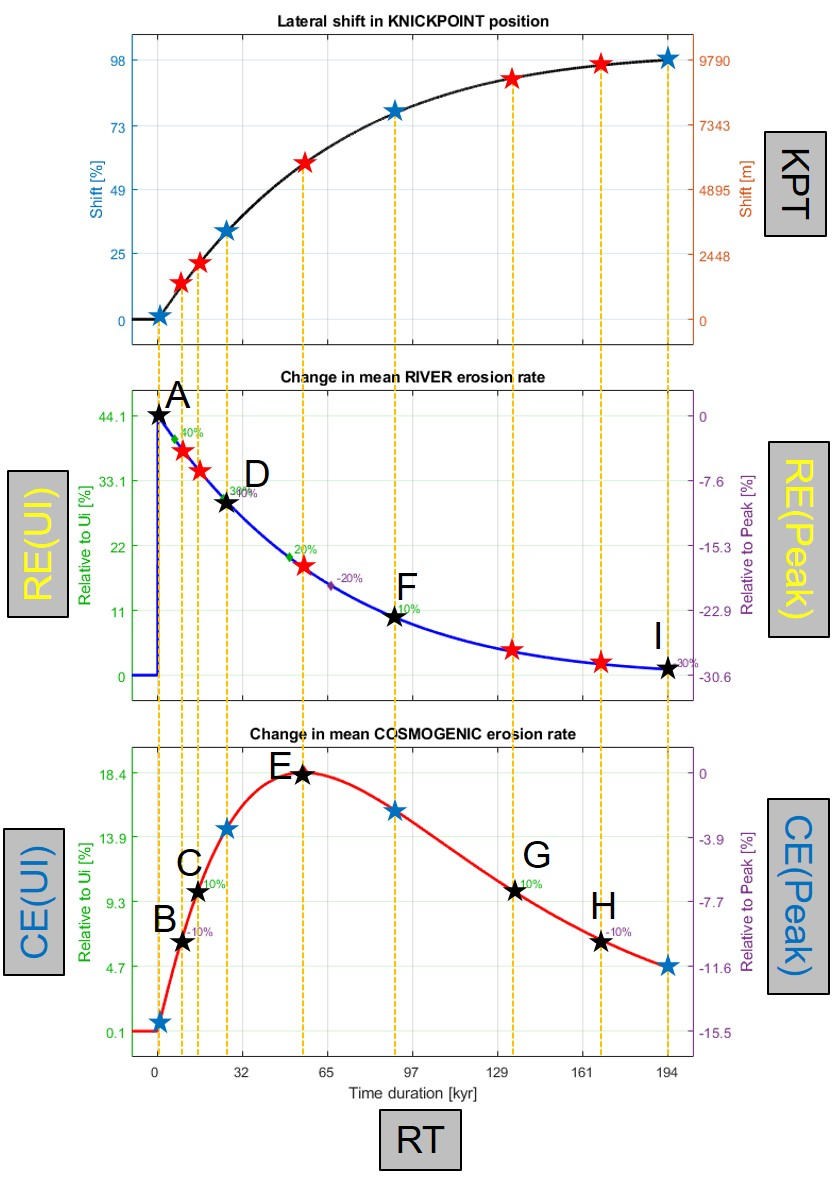
\includegraphics[width=1\textwidth]{profilehelp2.jpg}
    \caption[@ what point with label]{@ what point with label}
    \label{fig:RECEhelp2}    
\end{figure}

\begin{figure}[H]
    \centering
    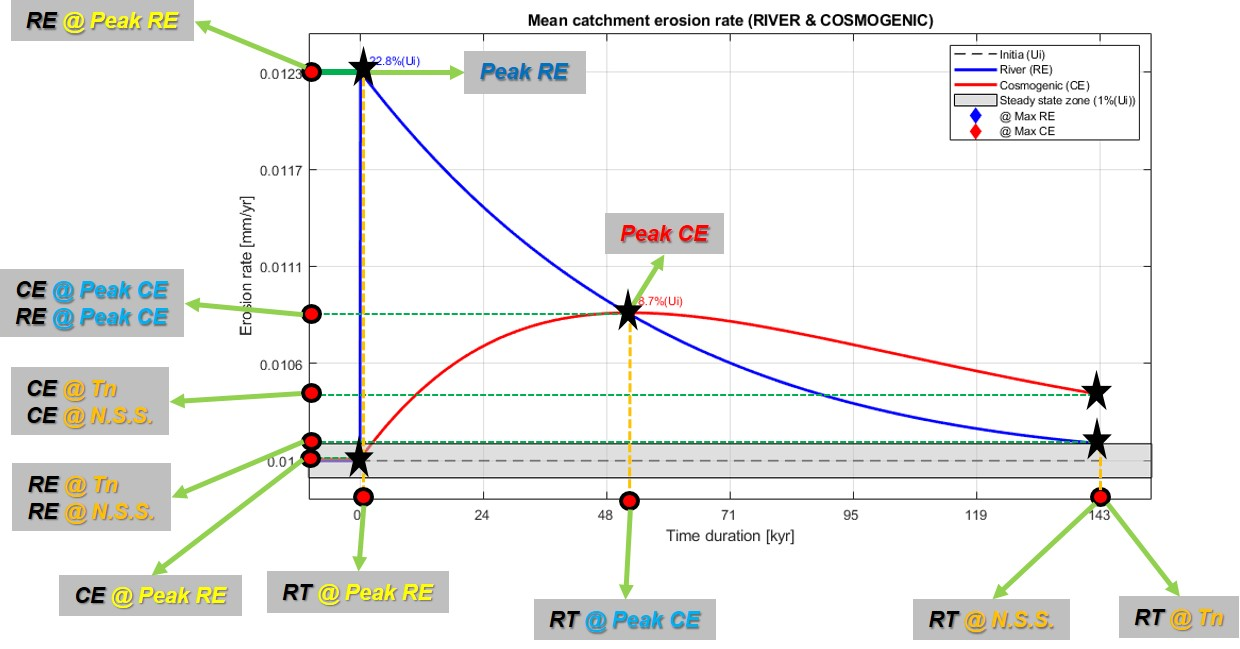
\includegraphics[width=1\textwidth]{profilehelp1.jpg}
    \caption[Mean catchment erosion rate with label]{Mean catchment erosion rate with label}
    \label{fig:RECEhelp1}    
\end{figure}

\section{Plot Histogram panel}
This panel plots two types of histograms. In order to use this panel, you select data from the data panel. It only considers the data inside the selected area (blue shadow).

\begin{figure}[H]
    \centering
    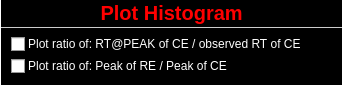
\includegraphics[width=0.45\textwidth]{plothist.png}
    \caption[Plot Histogram panel]{Plot Histogram panel}
    \label{fig:plothist}    
\end{figure}

\subsection{Response time histogram}

The first checkbox plots a histogram based on a ratio of two parameters related to the cosmogenic sample points (equation \ref{eq:hist1}). The "calculated RT @ Peak CE" is the calculated response time at the peak of the mean catchment cosmogenic erosion rate. The "observed RT" is the observed response time of the cosmogenic sample points measured in the lab. 

\begin{equation}
\frac{calculated RT @ Peak CE}{Obsereved RT}
\label{eq:hist1}
\end{equation}

This ratio can start from zero to very large values. Therefore we only limit the histogram between zero and two and the rest is shown in the top right of the figure as a string (figure \ref{fig:hist_RT}). All the blue bars smaller than one (red line) show the pixels with an observed response time greater than modeled response time.

\begin{figure}[H]
    \centering
    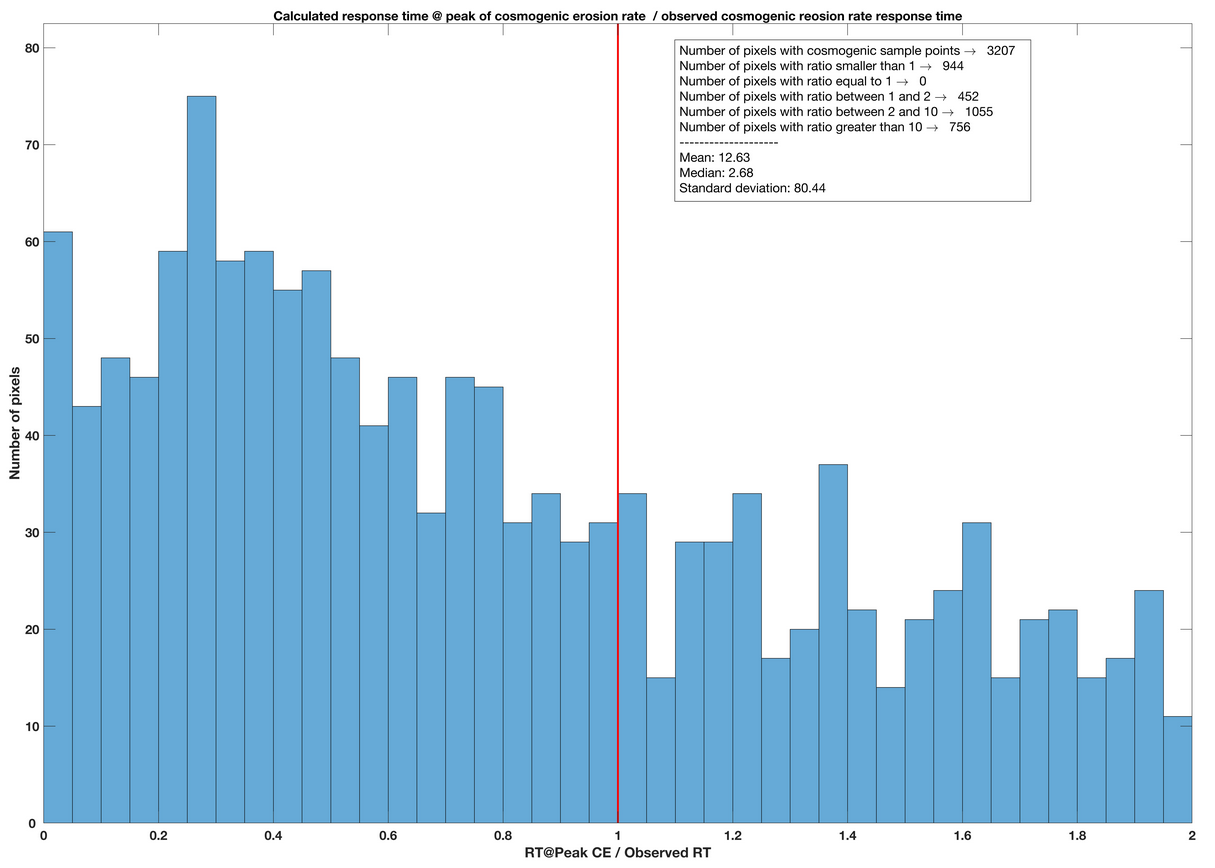
\includegraphics[width=0.6\textwidth]{hist_RT.png}
    \caption[Response time histogram]{Response time histogram}
    \label{fig:hist_RT}    
\end{figure}

\subsection{Erosion rate histogram}

The second checkbox plots a histogram based on a ratio of two parameters related to the value of river erosion rate and cosmogenic erosion rate (equation \ref{eq:hist2}). The "Peak RE" is the peak value of the mean catchment river erosion rate at each pixel. The "Peak CE" is the peak value of the mean catchment cosmogenic erosion rate at each pixel.

\begin{equation}
\frac{Peak RE}{Peak CE}
\label{eq:hist2}
\end{equation}

This histogram is usually limited between zero and two or sometimes a bit bigger. The absolute value of the "Peak RE" is always greater than the absolute value of "Peak CE". Therefore, if a pixel has a ratio greater than one, it means the shape of erosion change is the same as figure \ref{fig:profiletype_pos} (a positive profile). Also if a pixel has a ratio smaller than one, the erosion change has a shape like figure \ref{fig:profiletype_neg} (a negative profile).

\begin{figure}[H]
    \centering
    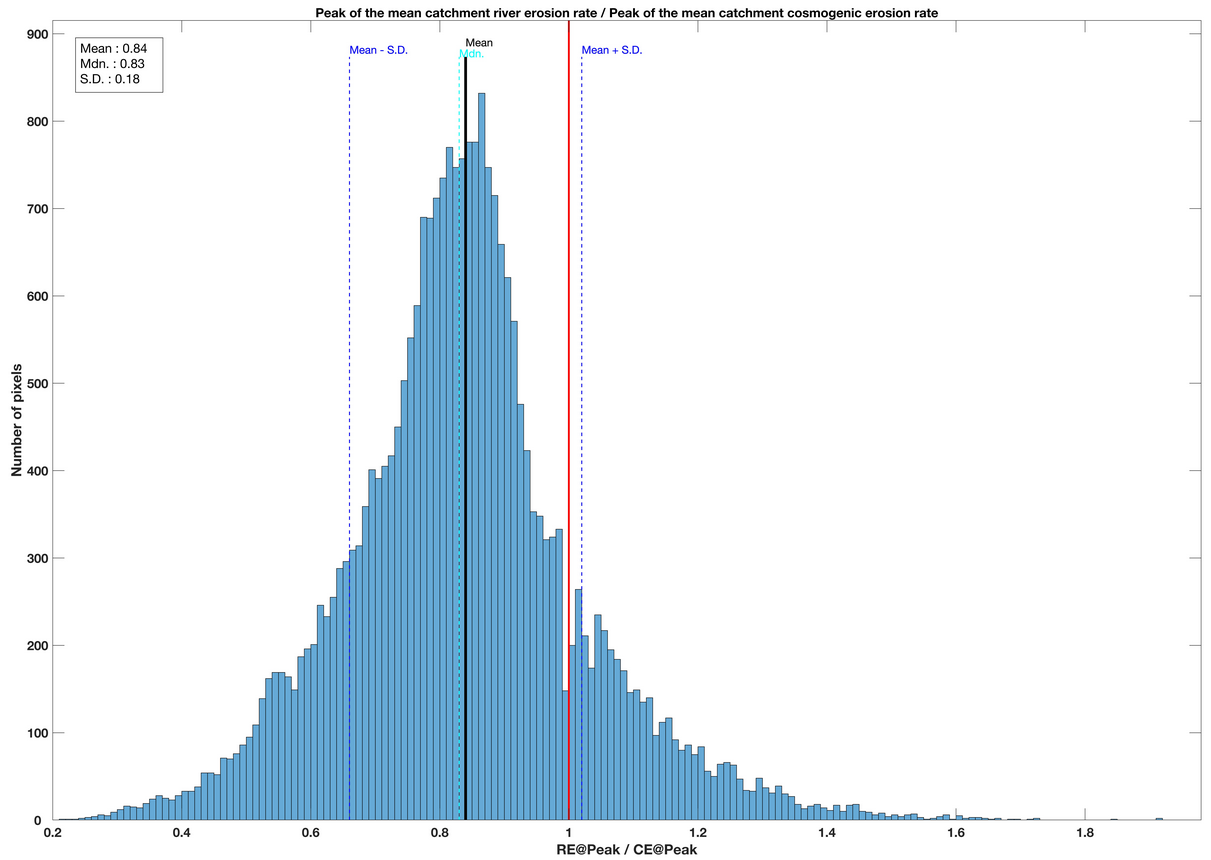
\includegraphics[width=0.6\textwidth]{hist_E.png}
    \caption[Erosion histogram]{Erosion histogram}
    \label{fig:hist_E}    
\end{figure}

\chapter{APPENDIX}\label{sec:apndx}
\section{BriefData header}
Here we explain the header of each column for BreifData matrix. As explained before this is the most important data file for the program and all the models which were made before are optimized and stored in this matrix. This matrix has 313 columns and below is the explanation of each column. First seven columns explained seperatley and the rest are explained with their abbreviations in figure \ref{fig:header}. For the abbreviations please refer to table \ref{tab:abbr} and table \ref{tab:@RT}.\\
\linebreak
1: Pixel number\\
2: Latitude\\
3: Longitude\\
4: Altitude\\
5: Initial precipitation\\
6: Final precipitation\\
7: End time (time when the model stops)\\

\begin{figure}[H]
    \centering
    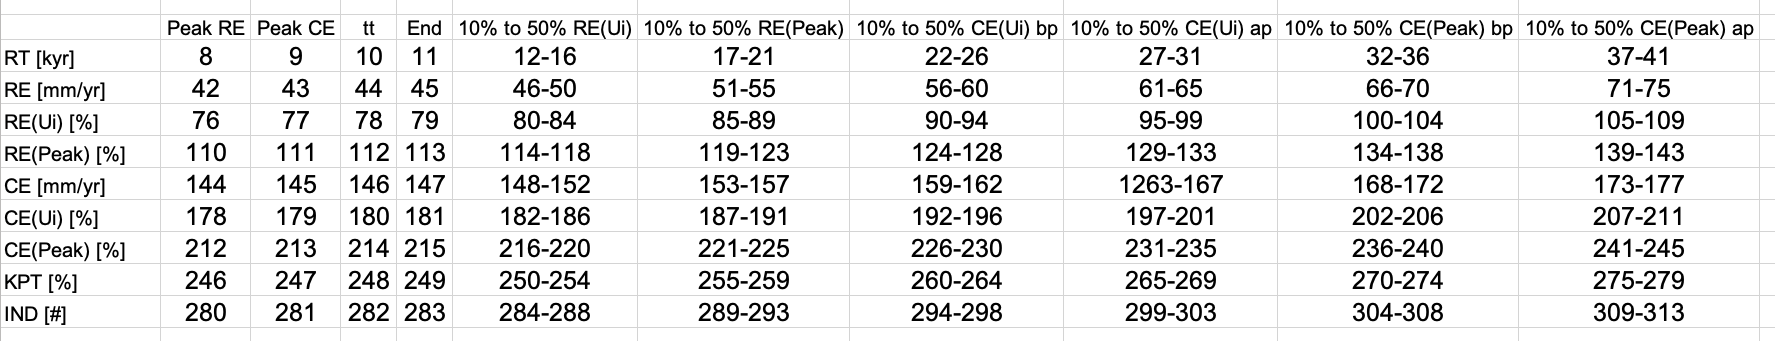
\includegraphics[width=1\textwidth]{header.png}
    \caption[BreifData Header]{BreifData Header}
    \label{fig:header}    
\end{figure}


\end{document}


8-41: RESPONSE TIME (RT)\\
8: RT @ Peak River Erosion rate\\
9: RT @ Peak Cosmogenic Erosion rate\\
10: RT @ Model duration (time duration between two geological time period)\\
11: RT @ Model end\\
12-16: RT @ 10\%,20\%,30\%,40\%50\% River Erosion rate relative to initial rock uplift rate\\
17-21: RT @ 10\%,20\%,30\%,40\%50\% River Erosion rate relative to its own peak\\
22-26: RT @ 10\%,20\%,30\%,40\%50\% Cosmogenic Erosion rate relative to initial rock uplift rate (before peak)\\
27-31: RT @ 10\%,20\%,30\%,40\%50\% Cosmogenic Erosion rate relative to initial rock uplift rate (after peak)\\
32-36: RT @ 10\%,20\%,30\%,40\%50\% Cosmogenic Erosion rate relative to its own peak (before peak)\\
37-41: RT @ 10\%,20\%,30\%,40\%50\% Cosmogenic Erosion rate relative to its own peak (after peak)\\

42-75: RESPONSE EROSION RATE (RE)\\
42: RT @ Peak River Erosion rate\\
43: RT @ Peak Cosmogenic Erosion rate\\
44: RT @ Model duration (time duration between two geological time period)\\
45: RT @ Model end\\
46-50: RT @ 10\%,20\%,30\%,40\%50\% River Erosion rate relative to initial rock uplift rate\\
51-55: RT @ 10\%,20\%,30\%,40\%50\% River Erosion rate relative to its own peak\\
56-60: RT @ 10\%,20\%,30\%,40\%50\% Cosmogenic Erosion rate relative to initial rock uplift rate (before peak)\\
61-65: RT @ 10\%,20\%,30\%,40\%50\% Cosmogenic Erosion rate relative to initial rock uplift rate (after peak)\\
32-36: RT @ 10\%,20\%,30\%,40\%50\% Cosmogenic Erosion rate relative to its own peak (before peak)\\
37-41: RT @ 10\%,20\%,30\%,40\%50\% Cosmogenic Erosion rate relative to its own peak (after peak)\\

76-109: RESPONSE EROSION RATE relative to Initial rock uplift rate (RE(Ui))\\
8: RT @ Peak River Erosion rate\\
9: RT @ Peak Cosmogenic Erosion rate\\
10: RT @ Model duration (time duration between two geological time period)\\
11: RT @ Model end\\
12-16: RT @ 10\%,20\%,30\%,40\%50\% River Erosion rate relative to initial rock uplift rate\\
17-21: RT @ 10\%,20\%,30\%,40\%50\% River Erosion rate relative to its own peak\\
22-26: RT @ 10\%,20\%,30\%,40\%50\% Cosmogenic Erosion rate relative to initial rock uplift rate (before peak)\\
27-31: RT @ 10\%,20\%,30\%,40\%50\% Cosmogenic Erosion rate relative to initial rock uplift rate (after peak)\\
32-36: RT @ 10\%,20\%,30\%,40\%50\% Cosmogenic Erosion rate relative to its own peak (before peak)\\
37-41: RT @ 10\%,20\%,30\%,40\%50\% Cosmogenic Erosion rate relative to its own peak (after peak)\\







%1:5 -------> Npixel , lat, long, Pi, Pn
%6:39 -------> RT
%40:73-------> RE
%74:107----------> RE(Ui)
%108:141 --------> RE(Peak)
%142:175 -------> CE
%176:209 -------> CE(Ui)
%210:243 -------> CE(Peak)
%244:277 -------->KPT
%275:
%    
%for each parameters @:
%6:9 -------> peak of RE, peak of CE, model duration, end of the model
%10:14 -------> 10,20,30,40,50 of RE(Ui)
%15:19 -------> 10,20,30,40,50 of RE(Peak)
%20:24 -------> 10,20,30,40,50 of CE(Ui) before peak
%25:29 -------> 10,20,30,40,50 of CE(Ui) after peak
%30:34 -------> 10,20,30,40,50 of CE(Peak) before peak
%35:39 ------->10,20,30,40,50 of CE(Peak) after peak